\documentclass[conference]{IEEEtran}

\usepackage[utf8]{inputenc}
\usepackage[T1]{fontenc}
\usepackage{silence}\WarningsOff[latexfont]

\usepackage{amsmath}

\RequirePackage{tikz}[2010/10/13]
\usetikzlibrary{arrows,automata,calc,intersections,patterns,decorations.pathmorphing,decorations.pathreplacing}

\usepackage{graphicx}
\usepackage{cite}
\usepackage{url}
\usepackage[caption=false,font=footnotesize]{subfig}
\usepackage[binary-units,per-mode=symbol]{siunitx}
\sisetup{list-final-separator = {, and }}
\usepackage{booktabs}
\usepackage{pifont}
\usepackage{microtype}
\usepackage{textcomp}
\usepackage[american]{babel}
\usepackage[noabbrev,capitalise]{cleveref}
\usepackage{xspace}
\usepackage{hyphenat}
\usepackage[draft,inline,nomargin,index]{fixme}
\fxsetup{theme=color}
\usepackage{grffile}
\usepackage{xfrac}
\usepackage{multirow}
\RequirePackage{xstring}
\RequirePackage{xparse}
\RequirePackage[index=true]{acro}

\NewDocumentCommand\acrodef{mO{#1}mG{}}{\DeclareAcronym{#1}{short={#2}, long={#3}, #4}}
\NewDocumentCommand\acused{m}{\acuse{#1}}

\usepackage{upquote}

\acrodef{i.i.d.}{independent identically distributed}
\DeclareMathOperator*{\argmax}{arg\!\max}

\begin{document}

\title{Characterization of a population parameters}
\author{
	\IEEEauthorblockN{Davide Pedranz, Mat. number 189295}
	\texttt{davide.pedranz@studenti.unitn.it}
}

\maketitle

\begin{abstract}
An electronic probe measures the output of a circuit which is known to generate independent identically distributed samples taken from a logistic distribution.
The probe is affected by a Gaussian white noise and a sinusoidal bias.
Given the measures data set, we want to estimate the mean and its confidence interval in order to decide whether to keep or discard the circuit.
\end{abstract}

\acresetall

\section{Introduction}
\label{sec:introduction}
Circuitry are widely used in every electronic device.
In order for those devices to work properly, high quality circuitry is needed.
The quality of a circuitry can be evaluated measuring some of its properties.
Unfortunately, each measurement is subject to some random noise or bias.
In order to achieve reliable results, the stochastic nature of the measuring process must be taken into account.

In this case, we have a circuitry which is known to generate \ac{i.i.d.} samples taken from a population with a logistic distribution.
The electronic probe used for the measures is known to introduce a white Gaussian noise and a sinusoidal bias.
The actual measures can thus be described as:

\begin{equation}
    \begin{gathered}
        x_{t} = A sin(2 \pi f t) + Y + Z, \\
        Y \sim Logis(\mu, s), \; Z \sim N(0, \sigma_{z}).
    \end{gathered}
    \label{eq:original-sample}
\end{equation}

Our aim is to estimate the five parameters of the model given the measures data set.
In particular, we are interested in the mean $\mu$ of the logistic distribution $Y$.
In addition, a confidence interval for the $\hat{\mu}$ is required.

The given data set contains $N = \num{60000}$ points from a sampling done at $ F = \SI{20}{\kilo\hertz}$ for \SI{3}{\second}.
We assume the frequency $f$ of the sinusoid to be an integer divisor of the sampling frequency and to be low, in the order of ten/hundreds of \SI{}{\hertz}.

We will estimate one parameter at a time, use it to clean the samples, then focus on the next one until the last one.
In particular, we will start from $\mu$, then estimate $f$ and $A$, and finally $s$ and $\sigma$.
As the last step, we will estimate the confidence interval for $\hat{\mu}$.

\section{First parameter - Mean $\mu$}
\label{sec:mean}

We start from the estimation of the mean $\mu$ of the logistic distribution $Y$.
We observe that:
\begin{itemize}
    \item the Gaussian $Z$ has zero mean, thus $E[Z] = 0$;
    \item the data set contains an integer number of periods of the sinusoid, which implies that its mean over the entire data set is zero $E[Asin(2 \pi f t)] = 0$.
\end{itemize}

Thus, we can build an unbiased estimator $\hat{\mu}$ by taking the average on the whole data set:

\begin{equation}
    \hat{\mu} = \frac{1}{n}\sum_{t=1}^{n}x_t = 3.00
    \label{eq:mean}
\end{equation}

It is easy to prove that $\hat{\mu}$ in \cref{eq:mean} is unbiased:

\begin{equation*}
    \begin{split}
        E[\hat{\mu}] &= E \Big[ \frac{1}{n}\sum_{t=1}^{n} \big( A sin(2 \pi f t) + Y + Z \big) \Big] \\
                     &= \frac{1}{n} \sum_{t=1}^{n} E[A sin(2 \pi f t)] + \frac{1}{n} n E[Y] + \frac{1}{n} n E[Z] \\
                     &= 0 + \mu + 0 = \mu.
    \end{split}
\end{equation*}

\section{Second Parameter - Frequency $f$}
\label{sec:frequency}

The second parameter in our estimation is the frequency $f$ of the sinusoid.
First, we clean the data set by subtracting the estimation of the mean $\mu$. 
The new data set has zero mean and can be described in a similar way to the original one in \cref{eq:original-sample}:

\begin{equation*}
    \begin{gathered}
        x_{t} = A sin(2 \pi f t) + Y + Z, \\
        Y \sim Logis(0, s), \; Z \sim N(0, \sigma_{z}).
    \end{gathered}
\end{equation*}

Since $Y$ and $Z$ are independent on each other and produce \ac{i.i.d.} samples, the correlation of the single random variables is caused only by the sinusoidal noise.
S0, we can use the autocorrelation function to estimate the frequency $f$.

The result of the autocorrelation on a sine function is a cosine with the same frequency, as shown by \cref{eq:autocorrelation}.

\begin{equation}
    \begin{split}
        R(\tau) &= E[A sin(2\pi ft) \cdot A sin(2\pi f(t+\tau))] \\
        &= \frac{1}{T_c} \int_{0}^{T_c} A^2(sin(2\pi f t) \cdot sin(2\pi f (t+\tau )) \, dt \\
        &= \frac{1}{T_c} \bigg[ A^2 \frac{1}{2} cos(2\pi ft) \; t + \frac{1}{8\pi f} sin(2\pi f(\tau+2t)) \; + \\
        &\;\;\;\;\; - \frac{1}{8\pi f} sin(2\pi f\tau) \bigg]_{t=0}^{t=T_c} \\
        &= \frac{1}{2} A^2 cos(2\pi f\tau)
    \end{split}
    \label{eq:autocorrelation}
\end{equation}

Note that $T_c$ is much greater than $\frac{1}{f}$, so it holds:
$$ sin(2 \pi f \tau) = sin(2 \pi f (\tau + 2 T_c)). $$

Using \cref{eq:autocorrelation}, we can compute the autocorrelation function on the data set:

\begin{equation}
    \begin{split}
    R(\tau) &= E[X(t)\cdot X(t+\tau)] \\
            &= \frac{1}{2} A^2 cos(2\pi f\tau) +  \operatorname{Var}[Y] + \operatorname{Var}[Z].
    \end{split}
\end{equation}

\begin{figure}[t]
	\centering
	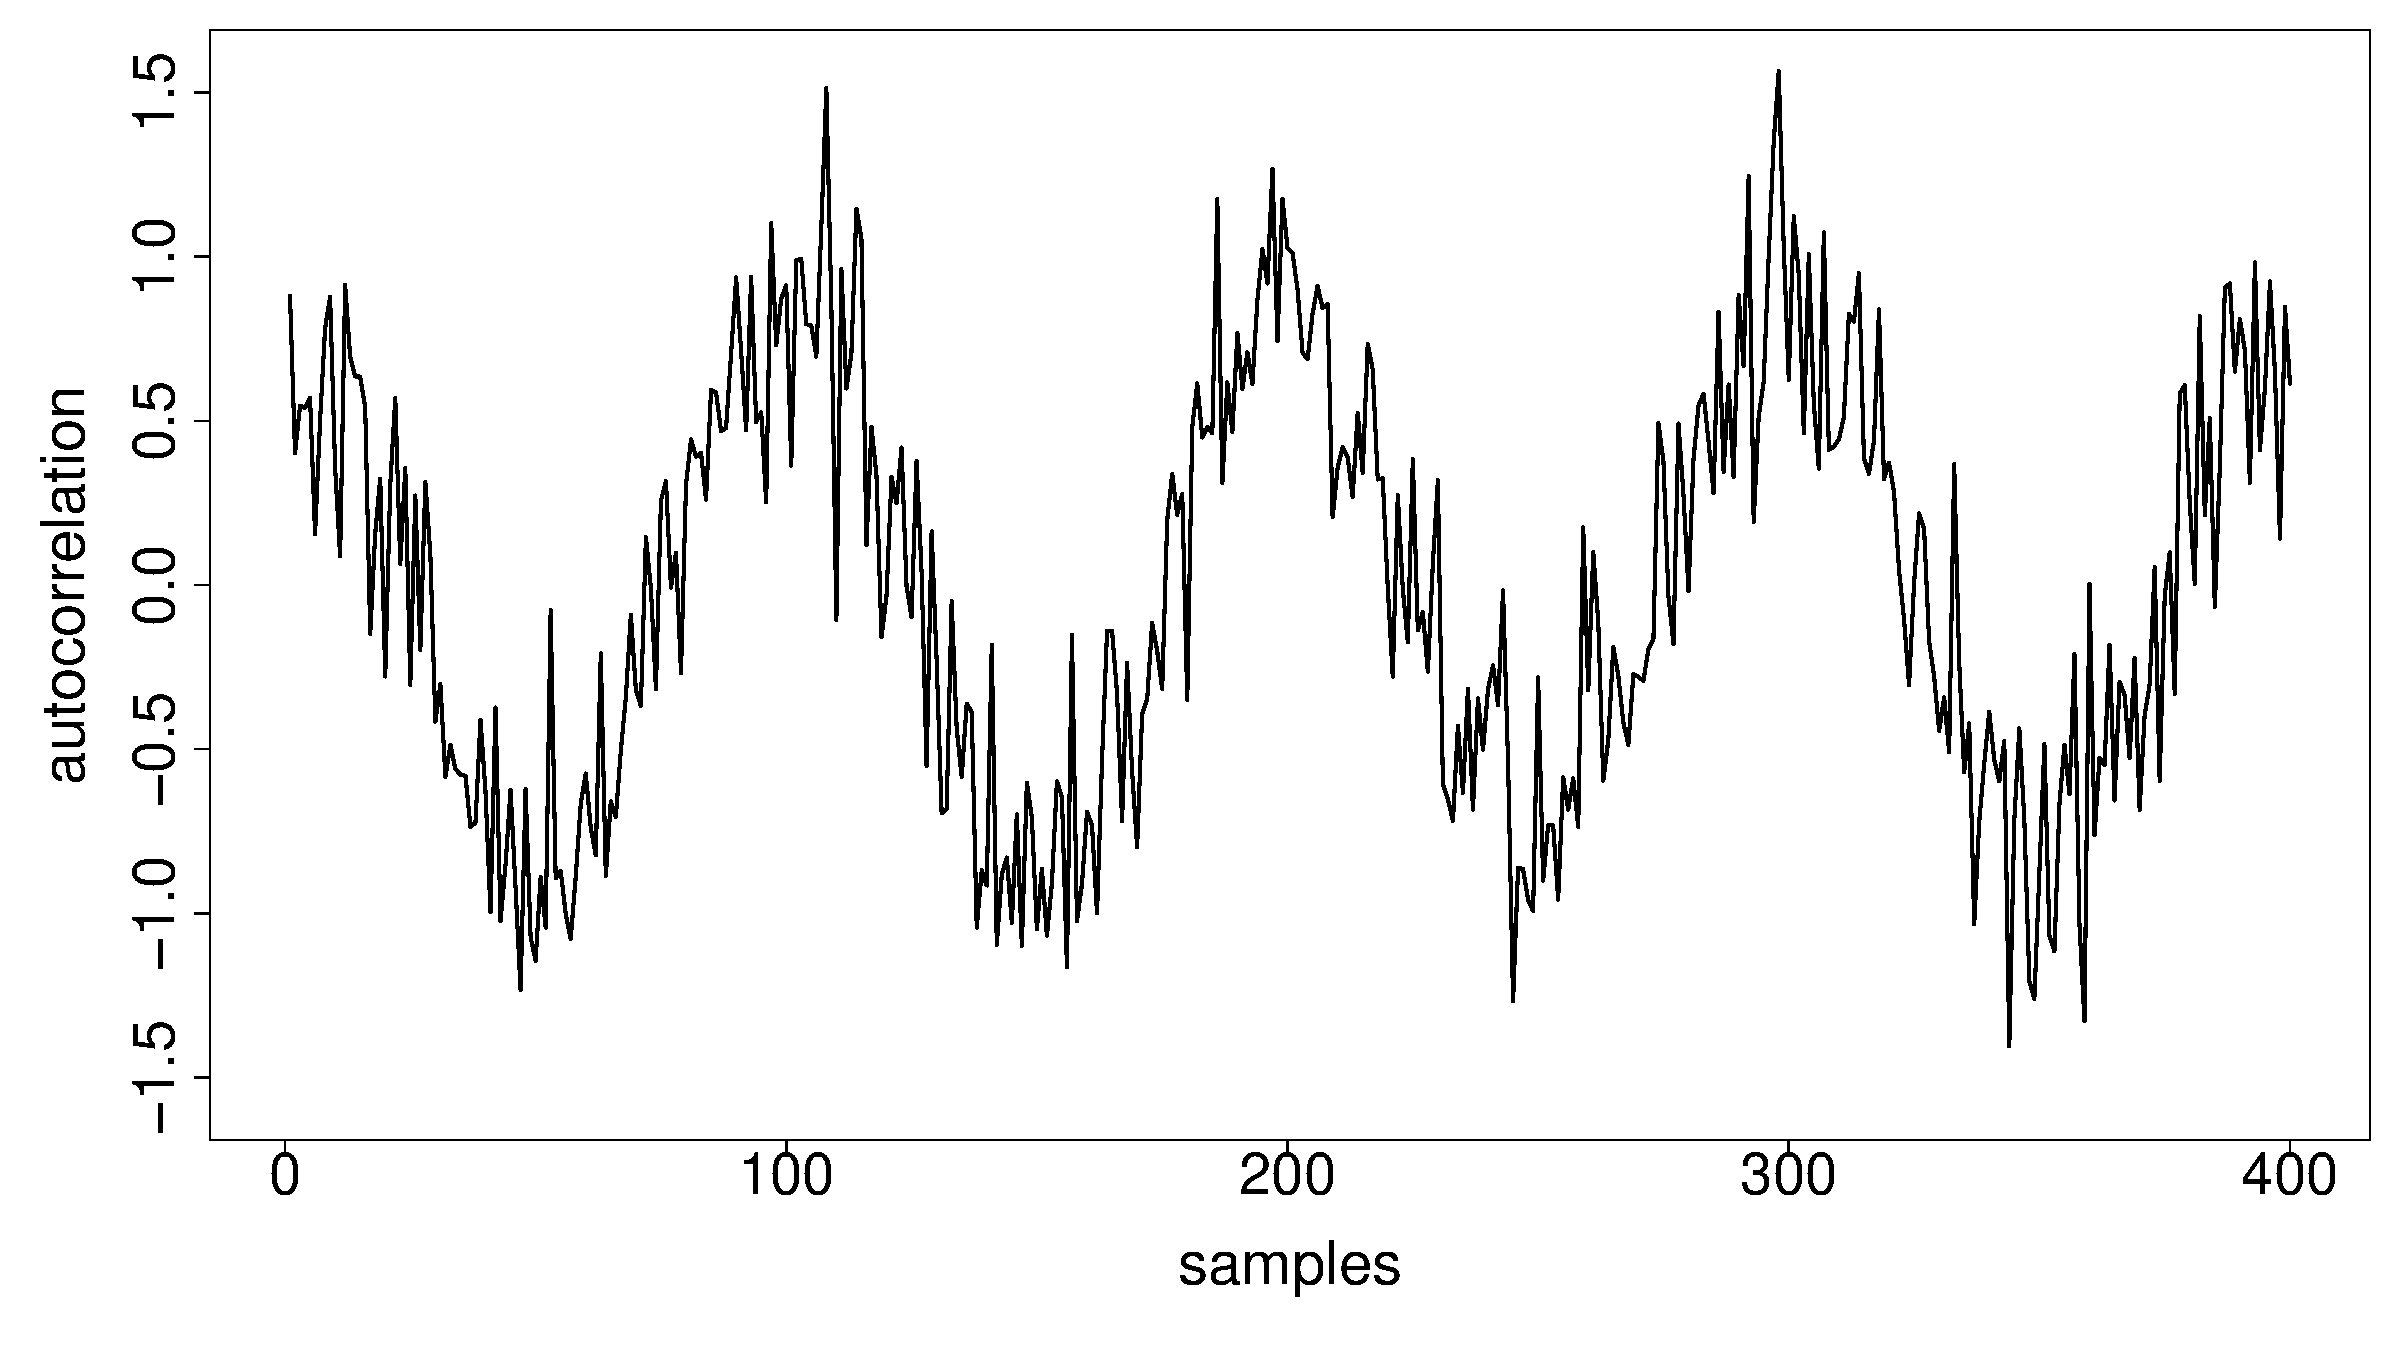
\includegraphics[width=\columnwidth]{figures/autocorrelation}
	\caption{Autocorrelation function of the first \num{400} points of the sample. It is easy to notice the underlying a cosine function.}
	\label{fig:autocorrelation}
\end{figure}

\cref{fig:autocorrelation} shows the autocorrelation function of the first \num{400} points of the data set.
As expected, the function has the shape of a cosine function.
The residual noise due to the variances of $Y$ and $Z$.

It is easy to see from the graph that each period of the sinusoid contains about \num{100} samples.
To get the precise number, we use a numerical approach.
We denote with $lag$ half of the period of the sinusoid.
For an interval of our rough estimation of the $lag$ (in this case \num{50}), we compute the average of the absolute value of the peaks (positive and negative) as a function of the lag's guess.
Then, we take the value that maximizes this function as the estimated lag.

\begin{equation*}
    lag = \argmax_{l} \sum_{\tau=1}^{\big\lfloor \frac{N}{2 \cdot l} \big\rfloor} |R(\tau + l)| + |R(\tau + 2 \cdot l)|
\end{equation*}

Now the frequency $f$ can be estimated as:

\begin{equation*}
    \hat{f} = \frac{F}{2 \cdot lag} = \frac{\SI{20}{\kilo\hertz}}{2 \cdot 50} = \SI{200}{\hertz}
\end{equation*}

\section{Third Parameter - Amplitude $A$}
\label{sec:amplitude}

The amplitude $A$ of the sinusoid can be computed in a similar way.
\cref{eq:autocorrelation} describe the relationship between the original sine signal and its autocorrelation function.
To estimate the amplitude of the autocorrelation function $A_{cos}$, we take the average of the absolute value of the theoretical highest and lowest points of each period of the cosine.
Formally:

\begin{equation}
    \begin{gathered}
        n = \Big\lfloor \frac{2 \cdot lag}{N} \Big\rfloor, \\
        A_{cos} = \frac{1}{n} \sum_{\tau=1}^{n} |R(\tau + lag)| + |R(\tau + 2 \cdot lag)| = 0.81
    \end{gathered}
\end{equation}

As for the case of the frequency, we take the mean over all peaks to reduce the noise due to the variances of $Y$ and $Z$.

Then, we can easily derive the estimation of the original amplitude $A$:

\begin{equation*}
    \hat{A} = \sqrt{2 \cdot A_{cos}} = 1.27.
\end{equation*}
\section{Last Parameters - $s$ and $\sigma_n$}
\label{sec:variances}

We remove the sinusoid from the data set by subtracting the theoretical sine function with frequency equal to the estimated frequency $f$ and amplitude equal to the estimated amplitude $A$.
Now the samples can be described as:

\begin{equation*}
    \begin{gathered}
        X = Y + Z, \\
        Y \sim Logis(0, s), \; Z \sim N(0, \sigma_{z}).
    \end{gathered}
\end{equation*}

To estimate the remaining parameters $s$ and $\sigma$, we can analyze the moments of $X = Y + Z$.

Both $Y$ and $Z$ have zero mean, so the first moment does not provide any useful information about the single distributions.

Since $Y$ and $Z$ are independent, the variance of the sum is equal to the sum of the variances, formally:

\begin{equation}
    \operatorname{Var}[Y+Z] = \operatorname{Var}[Y] + \operatorname{Var}[Z]
    \label{eq:variances}
\end{equation}

Both a logistic and a Gaussian distribution are symmetric with respect to the origin, so the skewness of $X$, $Y$ and $Z$ is zero.

The excess kurtosis of a Logistic distribution is always \num{1.2}, while the Gaussian distribution one is always \num{0}:

\begin{equation*}
    \operatorname{Kurt}[Y] - 3 = 1.2,\; \operatorname{Kurt}[Z] - 3 = 0.
\end{equation*}

We also know that the excess kurtosis of the sum of independent random variables for which the fourth moment exists has the following property, according to \cite{wiki:kurtosis}:

\begin{equation*}
    \operatorname{Kurt}[Y+Z] - 3 = \frac{\sigma_y^{\,4} (\operatorname{Kurt}[Y] - 3) + \sigma_z^{\,4} (\operatorname{Kurt}[Z] - 3)}{(\sigma_y^{\,2} + \sigma_z^{\,2})^2},
\end{equation*}

where $\sigma_y$ and $\sigma_z$ denote respectively the standard deviation of $Y$ and $Z$. We can thus compute the excess kurtosis of $X$:

\begin{equation}
    \operatorname{Kurt}[X] - 3 = \frac{1.2 \cdot \sigma_{y}^{\,4}}{(\sigma_{y}^{\,2} + \sigma_{z}^{\,2})^2}.
    \label{eq:kurtosis}
\end{equation}

From \cref{eq:variances} and \cref{eq:kurtosis} we obtain a system of two equations in two variables.
$\operatorname{Var}[X]$ and $\operatorname{Kurt}[X] - 3$ are computed on the data set using the standard well known estimators.
The system has two solutions, but we are interested only in the positive one.

\begin{equation*}
    \begin{cases}
        \hat{\sigma}_y^{\,2} = \sqrt{\frac{(\operatorname{Kurt}[X] - 3) \cdot \operatorname{Var}[X]^2}{1.2}} \\
        \hat{\sigma}_z^{\,2} = \operatorname{Var}[X] - \hat{\sigma}_y^{\,2}
    \end{cases}
\end{equation*}

The estimate of $s$ and $\sigma_z$ becomes now trivial:
\begin{equation*}
    \hat{s} = \frac{\hat{\sigma}_y}{\pi} \sqrt{3} = 4.49, \;\; \hat{\sigma}_z = 0.97.
\end{equation*}

\section{Mean Confidence Interval}
\label{sec:confidence}

The data set contains a sinusoidal noise, which makes the samples sample not identically distributed.
In order to compute a small confidence interval with a high probability, we need to transform the data set to obtain \ac{i.i.d.} samples.
The used technique is the batch means.

We observe that the mean operator is linear. This allows to compute the mean of the original data set by dividing the samples in batches of some fixed size, computing the mean of each batch and finally the mean of the means.

If we take the size of the batch as a multiple of the wavelength of the sinusoid and compute the batches, we obtain a population of random variables \ac{i.i.d.}, since the sum of any sinusoidal signal over a single period is zero.
Since the size is still high (\num{300} elements), we can treat the new population as normally distributed.
We computed two confidence intervals for a confidence of \num{95}\% and \num{99}\%:

\begin{equation}
    \begin{split}
        P[2.94 < \mu < 3.06] &= 0.95 \\
        P[2.92 < \mu < 3.08] &= 0.99    
    \end{split}
    \label{eq:confidence}
\end{equation}

A second possibility is to consider the data set without the sinusoidal noise.
Removing the sinusoidal signal is subject to some noise which increases the variance of the new data set.
On the other, we can directly treat the population as normally distributed and use the confidence intervals for a Gaussian population.
The result of the computation gives practically the same numbers as the batch means technique (the difference is less \num{e-10}).
The high number of samples probably compensate the extra noise introduces by the sinusoid's removal.

\section{Conclusion}
\label{sec:conclusion}

\begin{table}
	\centering
	\caption{Summary of the estimated parameters}
	\label{tab:summary}
	\begin{tabular}{l>{\raggedright}p{3cm}c}
    	\toprule
    		\multicolumn{2}{l}{parameter} & \multicolumn{1}{c}{value} \\
    	\midrule
    		$\mu$    & mean of the logistic $Y$  & 3.00              \\
    		$f$      & frequency of the sinusoid & \SI{200}{\hertz}  \\
    		$A$      & amplitude of the sinusoid & 1.27              \\
    		$s$      & scale of the logistic     & 0.49              \\
    		$\sigma$ & s.d. of the Gaussian      & 0.96              \\
    	\bottomrule
	\end{tabular}
\end{table}


In this work, we solved the problem of estimating the parameters of a given model using a sample of measures.
This type of analysis should be used for every measure that requires some reliability, since every probe is subject to somer random noise.

The estimated values for each parameter are summarized in \cref{tab:summary}.
The confidence intervals defined in \cref{eq:confidence} are reported below for completeness:
\begin{align*}
    P[2.94 < \mu < 3.06] &= 0.95 \\
    P[2.92 < \mu < 3.08] &= 0.99
\end{align*}

First, we estimated the value for the mean parameters, which was not affected by the others.
Secondly, we used the auto correlation function to isolate and remove the sinusoidal noise.
Thirdly, we exploited the different shapes and moments of the Gaussian and the logistic distribution to separate them from each other.
Finally, we computed a confidence interval for the mean using the technique of the batch means.


\bibliographystyle{IEEEtran}
\bibliography{references}

\end{document}
